\documentclass{article}[11pt]
\usepackage[frenchb,english]{babel}
\usepackage[T1]{fontenc}
\usepackage[utf8]{inputenc}
\usepackage{amsmath,amssymb,latexsym}
\usepackage{times}
\usepackage{float}
\usepackage[left=2cm,right=2cm,top=2cm,bottom=2cm]{geometry}
\frenchbsetup{StandardLists=true} % � inclure si on utilise \usepackage[french]{babel}
\usepackage{enumitem}
\usepackage{fancyhdr}
\usepackage{mathrsfs}
\usepackage{graphicx}
%\usepackage[Algorithme]{algorithm}
%\usepackage{algorithmic}
\usepackage{tikz}
\usepackage{tabularx}
\usetikzlibrary{shapes}
\pagestyle{fancy}
\newcommand{\tr}[1]{{\vphantom{#1}}^{\mathit t}{#1}} 
\renewcommand\headrulewidth{1pt}
\fancyhead[L]{Cours 1�re S}
\fancyhead[R]{Yoann Pietri}
\newcounter{theoremecounter}[subsection]
\usepackage{titlesec}
\setcounter{secnumdepth}{3}% enl�ve la num�rotation apr�s les sections
%\renewcommand\thechapter {\Roman{chapter}}

 \setlength{\parindent}{0pt}

\newcommand{\R}{\mathbb{R}}
\newcommand{\N}{\mathbb{N}}
\newcommand{\Q}{\mathbb{Q}}
\newcommand{\Z}{\mathbb{Z}}
\newcommand{\C}{\mathbb{C}}
\newcommand{\K}{\mathbb{K}}
\newcommand{\eqi}{\Leftrightarrow}
\titleformat{\subsubsection}
   {\normalfont\fontsize{11pt}{13pt}\selectfont\bfseries}% apparence commune au titre et au num�ro
   {\thesubsubsection}% apparence du num�ro
   {1em}% espacement num�ro/texte
   {}% apparence du titre

\tikzstyle{theobox} = [draw=black, very thick,
    rectangle, rounded corners, inner sep=10pt, inner ysep=20pt]
\tikzstyle{theotitle} =[fill=white, text=black,rounded corners,draw=black,very thick]

\usepackage{tkz-tab}

\fancyhead[L]{Sujet : La suite de Fibonacci}

\begin{document}
\center{\Large{Sujet : la suite de Fibonacci (correction)}}
\flushleft
\section*{I - Etude d'une fonction}
Dans la suite du sujet, on note $f$ la fonction définie pour tout $x$ par $$f(x) = x^2-x-1$$
\begin{enumerate}
\item Comme toutes les fonctions trinômes, $f$ est définie sur $\R$
\item On a $$\Delta = (-1)^2 -4 \times 1 \times (-1) = 5 > 0$$ Ainsi $f$ possède deux racines réelles $$x_1 = \dfrac{1 + \sqrt{5}}{2}$$ et $$x_1 = \dfrac{1 - \sqrt{5}}{2}$$ 
\item Le coefficient dominant de $f$ est positif donc le trinôme est négatif entre les racines 
\begin{tikzpicture}
   \tkzTabInit{$x$ / 1 , $f$ / 1}{$-\infty$,$\dfrac{1-\sqrt{5}}{2}$,$\dfrac{1+\sqrt{5}}{2}$, $+\infty$}
   \tkzTabLine{, +,z,-,z, +,}
\end{tikzpicture}
\item $f$ est dérivable sur $\R$ et pour tout $x\in \R$, $$f'(x) =  2x-1$$
Ainsi on peut dresser le tableau de signe de $f'$ puis le tableau de variation de $f$\newline
\begin{tikzpicture}
   \tkzTabInit{$x$ / 1 , $f'(x)$ / 1, $f(x)$ / 1.5}{$-\infty$, $\frac{1}{2}$, $+\infty$}
   \tkzTabLine{, -, z,+ ,}
   \tkzTabVar{+/, -/ $-\frac{3}{2}$, +/}
\end{tikzpicture}\newline
\item Courbe représentative de $f$ \newline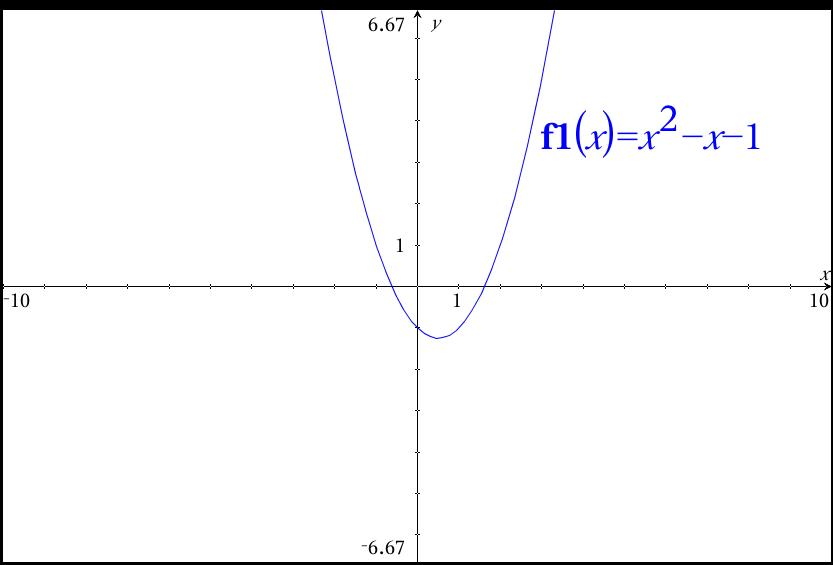
\includegraphics[scale=0.3]{fibo_ill1.jpg} 
\item La première manière est la manière calculatoire (et chiante)
$$\varphi^2 = \left(\dfrac{1+\sqrt{5}}{2}\right)^2 = \dfrac{1+2\sqrt{5}+5}{4} = \dfrac{3+\sqrt{5}}{2}$$ or $$\varphi +1 = \dfrac{1+\sqrt{5}}{2} + 1 = \dfrac{3+\sqrt{5}}{2}$$ La deuxième méthode constiste à dire que $\varphi$ est racine de $f$ donc $$f(\varphi)=0$$
$$\varphi^2-\varphi-1 = 0$$
$$\boxed{\varphi^2 = \varphi +1}$$
\item On a
$$\varphi^2 = \varphi +1$$ et $\varphi \neq 0$ donc par division par $\varphi$, 
$$\varphi = 1 + \dfrac{1}{\varphi}$$
$$\boxed{\dfrac{1}{\varphi} = \varphi -1}$$
\item La limite de $(u_{n+1})$ est la même que celle de $(u_n)$
\item Par passage à la limite dans 
$$u_{n+1} = 1 + \dfrac{1}{u_n}$$
on obtient 
$$\ell = 1 + \dfrac{1}{\ell}$$
d'où 
$$\ell^2 = \ell + 1$$
d'où $\ell = \varphi$ ou $\ell = \psi$\newline 
On a, pour tout $n\in \N$, $u_n \geq 0$ donc $\ell \geq 0$ donc $$\boxed{\ell = \varphi}$$
\item On a 
$$u_{50} = \dfrac{2036501174}{12586269025}\simeq 1,6180339887499$$
or 
$$\varphi \simeq 1,6180339887499$$ soit une correspondance totale sur tous les chiffres après la virgule que peut afficher ma calculatrice
\end{enumerate}
\section*{II - Quelques résultats sur les rationnels et les irrationnels}
\begin{enumerate}
\item Soient $x = \dfrac{p}{q}$ et $y = \dfrac{p'}{q'}$ avec $p,p' \in \Z$ et $q,q' \in \N^*$. Alors $$xy = \dfrac{pp'}{qq'}$$ et $pp' \in \Z$ et $qq' \in \N^*$ donc $xy \in \Q$
\item Soient $x = \dfrac{p}{q}$ et $y = \dfrac{p'}{q'}$ avec $p,p' \in \Z$ et $q,q' \in \N^*$. Alors $$x+y = \dfrac{p}{q} + \dfrac{p'}{q'} = \dfrac{pq' + p'q}{qq'}$$ et $pq'+ p'q \in \Z$ et $qq' \in \N^*$ donc $x+y \in \Q$
\item Soit $x = \dfrac{p}{q} \neq 0$ un rationnel ($p \in \Z^*$, $q\in N^*$ $$\dfrac{1}{x} = \dfrac{q}{p}$$
Si $p > 0$ c'est gagné, sinon si $p<0$, on remarque juste que $$\dfrac{q}{p} = \dfrac{-q}{-p}$$ et les signes sont rétablis
\item Supposons par l'absurde que $a\times b$ soit rationnel. Alors il le resterait par multiplication par $\dfrac{1}{b}$ d'après la question précédente et la question 1. Alors $a\times b\times \dfrac{1}{b}$ serait rationnel donc $a$ serait rationnel. Contradiction : $a\times b$ est irrationnel
\item Supposons par l'absurde que $a+b$ soit rationnel. Alors il le resterait quand on lui ajoute $-b$ ($-b$ est bien rationnel donc c'est bon d'après la question $2$) du coup $a + b -b$ est rationnel d'où $a$ rationnel : contradiction : $a+b$ est irrationnel
\item Pas forcément : si $a$ ets irrationnel, $-a$ l'est aussi et donc $a-a = 0 \in \Q$
\item Toujours pas forcément : on le montre à la question d'après, $\sqrt{2}$ est irrationnel et $\sqrt{2} \times \sqrt{2} = 2 \in \Q$
\item Soit $n$ un nombre impair. Il s'écrit $n = 2k+1$. Or $$(2k+1)^2 = 4k^2 + 4k +1 = 2(2k^2+2k)+1 = 2k'+1$$ avec $k' \in \N$ d'où $n^2$ impair. Le raisonnement s'appelle le raisonnement par contraposée
\item On va montrer que $\sqrt{2}$ est irrationnel. On suppose par l'absurde que $\sqrt{2}$ est irrationnel et donc on suppose l'existence de $p \in \N^*$ et $q \in \N^*$ tel que $$\sqrt{2} = \dfrac{p}{q}$$ avec $p$ et $q$ premiers entre eux
\begin{enumerate}
\item On sait que $\sqrt{2} \simeq 1,414 > 0$ ce qui donne $p>0$
\item Il suffit d'élever la relation précédente au carré : $$\left(\dfrac{p}{q}\right)^2 = \sqrt{2}^2$$
$$\dfrac{p^2}{q^2} = 2$$
$$p^2 = 2q^2$$
On déduit alors que $p^2$ est pair puis $p$ pair grâce à la question 8
\item $p$ est pair donc s'écrit $p = 2k$. Ainsi 
$$p^2 = 2q^2$$
$$4k^2 = 2q^2$$
puis par division par 2
$$2k^2 = q^2$$
On déduit alors que $q^2$ est pair puis $q$ pair toujours grâce à la question 8
\item On avait supposer que $p$ et $q$ étaient premiers entre eux (pgcd($p$,$q) = 1$) or on vient de montrer qu'il admettait deux comme diviseur commun (ou encore que pgcd($p$,$q) geq 2$)
\end{enumerate}
\item $$\varphi =  \dfrac{1+\sqrt{5}}{2}$$ donc c'est la somme d'un rationnel $\left(\dfrac{1}{2}\right)$ et d'un irrationnel $\left(\dfrac{\sqrt{5}}{2}\right)$ d'où $\varphi$ est irrationnel
\end{enumerate}
\section*{III - Suites récurrentes linéaires d'ordre 1}
Soit $a$ et $b$ deux réels. On s'interesse aux suites définies par $$\left\lbrace \begin{array}{l}
u_0 = u_0 \quad (\text{donné})\\
\forall n \in \N, u_{n+1} = au_n +b
\end{array}
\right.$$
\begin{enumerate}
\item Dans le cas $a=1$, $(u_n)$ est une suite arithmétique de raison $b$. Le terme général est alors $$u_n = u_0 + nb$$ et la limite est $+\infty$ si $b>0$, $-\infty$ si $b<0$ et $u_0$ si $b=0$
\item On a 
$$\dfrac{v_{n+1}}{v_n} = \dfrac{au_n+b - \dfrac{b}{1-a}}{u_n - \dfrac{b}{1-a}}$$
$$\dfrac{v_{n+1}}{v_n}  = a \dfrac{u_n + \dfrac{b}{a} - \dfrac{b}{1-a}}{u_n - \dfrac{b}{a(1-a)}}$$
$$\dfrac{v_{n+1}}{v_n}  = a \dfrac{u_n + b\left(\dfrac{1}{a} -\dfrac{1}{1-a}\right)}{u_n - \dfrac{b}{a(1-a)}}$$
$$\dfrac{v_{n+1}}{v_n}  = a \dfrac{u_n + b\left(\dfrac{1-a}{a(1-a)} -\dfrac{1}{a(1-a)}\right)}{u_n - \dfrac{b}{1-a}}$$
$$\dfrac{v_{n+1}}{v_n}  = a \dfrac{u_n + b\left(\dfrac{-a}{a(1-a)}\right)}{u_n - \dfrac{b}{1-a}}$$
$$\dfrac{v_{n+1}}{v_n}  = a \dfrac{u_n + \dfrac{-b}{1-a}}{u_n - \dfrac{b}{1-a}}$$
$$\dfrac{v_{n+1}}{v_n}  = a $$
On déduit que $(v_n)$ est géométrique de raison $a$ et de premier terme $$v_0 = u_0 - \dfrac{b}{1-a}$$
\item On a ainsi, pour tout $n\in \N$, 
$$\boxed{v_n = v_0 a^n =\left(u_0-\dfrac{b}{1-a}\right)a^n}$$
Puis 
$$u_n = v_n + \dfrac{b}{1-a}$$
$$\boxed{u_n = \left(u_0-\dfrac{b}{1-a}\right)a^n + \dfrac{b}{1-a}}$$
\item On a $0<a<1$ donc 
$$v_n\underset{n \rightarrow \infty}{\longrightarrow} 0$$
d'ou
$$\boxed{u_n\underset{n \rightarrow \infty}{\longrightarrow} \dfrac{b}{1-a}}$$
\end{enumerate}
\section*{IV - Suites récurrentes linéaires d'ordre 2}
Soit $a$ et $b$ dans $\R$. On dit qu'une suite $u_n$ vérifie $E_{(a,b)}$ si pour tout $n\in \N$, 
$$u_{n+2} = au_{n+1} + bu_n$$
De plus on note 
$$g_{(a,b)} : x\mapsto x^2-ax-b$$ et on note $\Delta_{(a,b)}$ son discriminant
\begin{enumerate}
\item Avec le résultat admis, 
$$u_0 = \lambda r_1^0 + \mu r_2^0$$
$$\boxed{u_0 = \lambda + \mu}$$
De plus 
$$u_1 = \lambda r_1^1 + \mu r_2^1$$
$$\boxed{u_1 = \lambda r_1 + \mu r_2}$$
On résout alors le système 
$$\left\lbrace\begin{array}{l}
u_0 = \lambda + \mu \quad(1)\\
u_1 = \lambda r_1 + \mu r_2 \quad(2)\\
\end{array}\right.$$
En faisant $(2) - r_2(1)$, on obtient 
$$u_1 - r_2u_0 = \lambda (r_1 - r_2)$$
$$\boxed{\lambda = \dfrac{u_1-r_2u_0}{r_1-r_2}}$$
($r_1-r_2 \neq 0$ car les racines sont distinctes)\newline

De même, en faisant $(2) - r_1 (1)$, on obtient 
$$\boxed{\mu = \dfrac{u_1-r_1u_0}{r_2-r_1}}$$
\item Avec le résultat admis, 
$$u_0 = (\lambda + \mu\times 0)r_0^0$$
$$\boxed{u_0 = \lambda}$$
De plus 
$$u_1 = (\lambda + \mu\times 1) r_0^1$$
$$u_1 = (u_0 + \mu)r_0$$
d'ou finalement
$$\boxed{\mu = \dfrac{u_1}{r_0} - u_0}$$
\end{enumerate}
\section*{V - Suite de Fibonacci}
On définit la suite de Fibonacci $(\mathcal{F}_n)$ par 
$$\left\lbrace \begin{array}{l}
u_0 = 0 \\
u_1 = 1\\
\forall n \in \N, \mathcal{F}_{n+2} = \mathcal{F}_{n+1} + \mathcal{F}_n
\end{array}
\right.$$
\begin{enumerate}
\item Les 11 premiers termes de la suite de Fibonacci
\begin{tabularx}{\linewidth}{|X|X|X|X|X|X|X|X|X|X|X|X|}
\hline 
$n$ & 0 & 1 & 2 & 3 & 4 & 5 & 6 & 7 & 8 & 9 & 10 \\ 
\hline 
$\mathcal{F}_n$ & 0 & 1 & 1 & 2 & 3 & 5 & 8 & 13 & 21 & 34 & 55 \\ 
\hline 
\end{tabularx} 
\item En fait on se retrouve avec une suite linéaire récurrence d'ordre 2, avec $a=1$ et $b=1$. Il faut trouver les racines de $g_{(1,1)}$. Or $g_{(1,1)} = f$ (comme les sujets sont bien faits...) et a deux racines distintces : $\varphi$ et $\psi$. Ainsi, pour tout $n\in \N$, 
$$\mathcal{F}_n = \lambda \varphi^n + \mu \psi^n$$
avec 
$$\lambda = \dfrac{1-\psi\times 0}{\varphi-\psi}$$
or $\varphi = \dfrac{1+\sqrt{5}}{2}$, $\psi = \dfrac{1-\sqrt{5}}{2}$d'où $\varphi - \psi = \sqrt{5}$ donc $$\lambda = \dfrac{1}{\sqrt{5}}$$
On a aussi 
$$\mu = \dfrac{1-r_1\times 0}{\psi-\varphi}$$
$$\mu = -\dfrac{1}{\sqrt{5}}$$
On déduit la formule de Binet, 
$$\mathcal{F}_n = \dfrac{1}{\sqrt{5}}\left(\varphi^n - \psi^n\right)$$
\item On a $$\dfrac{\mathcal{F}_{n+1}}{\mathcal{F}_n} = \dfrac{\varphi^{n+1} - \psi^{n+1}}{\varphi^{n} - \psi^n}$$
or $\psi^n \underset{n\rightarrow +\infty}{\longrightarrow} 0$ car $|\psi| <1$ d'où  $$\dfrac{\mathcal{F}_{n+1}}{\mathcal{F}_n} \underset{n \rightarrow \infty}{\longrightarrow} \varphi$$
\item $\dfrac{\mathcal{F}_{10}}{\mathcal{F}_{9}} \simeq 1,61765$. On peut aussi avoir une valeur approché de $\varphi$ : 
$\varphi \simeq 1,61803$. On a une convergence assez rapide (2 décimales après la virgule pour seulement 11 termes à calculer, c'est pas mal)
\end{enumerate}
\end{document}